%%%%%%%%%%%%%%%%%%%%%%%%%%%%%%%%%%%%%%%%%
%  My documentation report
%  Objetive: Explain what I did and how, so someone can continue with the investigation
%
% Important note:
% Chapter heading images should have a 2:1 width:height ratio,
% e.g. 920px width and 460px height.
%
%%%%%%%%%%%%%%%%%%%%%%%%%%%%%%%%%%%%%%%%%

%----------------------------------------------------------------------------------------
%	PACKAGES AND OTHER DOCUMENT CONFIGURATIONS
%----------------------------------------------------------------------------------------

\documentclass[11pt,fleqn]{book} % Default font size and left-justified equations

\usepackage[top=3cm,bottom=3cm,left=3.2cm,right=3.2cm,headsep=10pt,letterpaper]{geometry} % Page margins

\usepackage{xcolor} % Required for specifying colors by name
\definecolor{darkgreen}{RGB}{0, 153, 0} % Define the orange color used for highlighting throughout the book

% Font Settings
\usepackage{avant} % Use the Avantgarde font for headings
%\usepackage{times} % Use the Times font for headings
\usepackage{mathptmx} % Use the Adobe Times Roman as the default text font together with math symbols from the Sym­bol, Chancery and Com­puter Modern fonts

\usepackage{microtype} % Slightly tweak font spacing for aesthetics
\usepackage[utf8]{inputenc} % Required for including letters with accents
\usepackage[T1]{fontenc} % Use 8-bit encoding that has 256 glyphs

% Bibliography
\usepackage[style=alphabetic,sorting=nyt,sortcites=true,autopunct=true,babel=hyphen,hyperref=true,abbreviate=false,backref=true,backend=biber]{biblatex}
\addbibresource{bibliography.bib} % BibTeX bibliography file
\defbibheading{bibempty}{}

%----------------------------------------------------------------------------------------
%	VARIOUS REQUIRED PACKAGES
%----------------------------------------------------------------------------------------

\usepackage{titlesec} % Allows customization of titles

\usepackage{graphicx} % Required for including pictures
\graphicspath{{Pictures/}} % Specifies the directory where pictures are stored

\usepackage{lipsum} % Inserts dummy text

\usepackage{tikz} % Required for drawing custom shapes

\usepackage[english]{babel} % English language/hyphenation

\usepackage{enumitem} % Customize lists
\setlist{nolistsep} % Reduce spacing between bullet points and numbered lists

\usepackage{booktabs} % Required for nicer horizontal rules in tables

\usepackage{eso-pic} % Required for specifying an image background in the title page

%----------------------------------------------------------------------------------------
%	MAIN TABLE OF CONTENTS
%----------------------------------------------------------------------------------------

\usepackage{titletoc} % Required for manipulating the table of contents

\contentsmargin{0cm} % Removes the default margin
% Chapter text styling
\titlecontents{chapter}[1.25cm] % Indentation
{\addvspace{15pt}\large\sffamily\bfseries} % Spacing and font options for chapters
{\color{darkgreen!60}\contentslabel[\Large\thecontentslabel]{1.25cm}\color{darkgreen}} % Chapter number
{}  
{\color{darkgreen!60}\normalsize\sffamily\bfseries\;\titlerule*[.5pc]{.}\;\thecontentspage} % Page number
% Section text styling
\titlecontents{section}[1.25cm] % Indentation
{\addvspace{5pt}\sffamily\bfseries} % Spacing and font options for sections
{\contentslabel[\thecontentslabel]{1.25cm}} % Section number
{}
{\sffamily\hfill\color{black}\thecontentspage} % Page number
[]
% Subsection text styling
\titlecontents{subsection}[1.25cm] % Indentation
{\addvspace{1pt}\sffamily\small} % Spacing and font options for subsections
{\contentslabel[\thecontentslabel]{1.25cm}} % Subsection number
{}
{\sffamily\;\titlerule*[.5pc]{.}\;\thecontentspage} % Page number
[] 

%----------------------------------------------------------------------------------------
%	MINI TABLE OF CONTENTS IN CHAPTER HEADS
%----------------------------------------------------------------------------------------

% Section text styling
\titlecontents{lsection}[0em] % Indendating
{\footnotesize\sffamily} % Font settings
{}
{}
{}

% Subsection text styling
\titlecontents{lsubsection}[.5em] % Indentation
{\normalfont\footnotesize\sffamily} % Font settings
{}
{}
{}
 
%----------------------------------------------------------------------------------------
%	PAGE HEADERS
%----------------------------------------------------------------------------------------

\usepackage{fancyhdr} % Required for header and footer configuration

\pagestyle{fancy}
\renewcommand{\chaptermark}[1]{\markboth{\sffamily\normalsize\bfseries\chaptername\ \thechapter.\ #1}{}} % Chapter text font settings
\renewcommand{\sectionmark}[1]{\markright{\sffamily\normalsize\thesection\hspace{5pt}#1}{}} % Section text font settings
\fancyhf{} \fancyhead[LE,RO]{\sffamily\normalsize\thepage} % Font setting for the page number in the header
\fancyhead[LO]{\rightmark} % Print the nearest section name on the left side of odd pages
\fancyhead[RE]{\leftmark} % Print the current chapter name on the right side of even pages
\renewcommand{\headrulewidth}{0.5pt} % Width of the rule under the header
\addtolength{\headheight}{2.5pt} % Increase the spacing around the header slightly
\renewcommand{\footrulewidth}{0pt} % Removes the rule in the footer
\fancypagestyle{plain}{\fancyhead{}\renewcommand{\headrulewidth}{0pt}} % Style for when a plain pagestyle is specified

% Removes the header from odd empty pages at the end of chapters
\makeatletter
\renewcommand{\cleardoublepage}{
\clearpage\ifodd\c@page\else
\hbox{}
\vspace*{\fill}
\thispagestyle{empty}
\newpage
\fi}

%----------------------------------------------------------------------------------------
%	THEOREM STYLES
%----------------------------------------------------------------------------------------

\usepackage{amsmath,amsfonts,amssymb,amsthm} % For math equations, theorems, symbols, etc

\newcommand{\intoo}[2]{\mathopen{]}#1\,;#2\mathclose{[}}
\newcommand{\ud}{\mathop{\mathrm{{}d}}\mathopen{}}
\newcommand{\intff}[2]{\mathopen{[}#1\,;#2\mathclose{]}}
\newtheorem{notation}{Notation}[chapter]

%%%%%%%%%%%%%%%%%%%%%%%%%%%%%%%%%%%%%%%%%%%%%%%%%%%%%%%%%%%%%%%%%%%%%%%%%%%
%%%%%%%%%%%%%%%%%%%% dedicated to boxed/framed environements %%%%%%%%%%%%%%
%%%%%%%%%%%%%%%%%%%%%%%%%%%%%%%%%%%%%%%%%%%%%%%%%%%%%%%%%%%%%%%%%%%%%%%%%%%
\newtheoremstyle{ocrenumbox}% % Theorem style name
{0pt}% Space above
{0pt}% Space below
{\normalfont}% % Body font
{}% Indent amount
{\small\bf\sffamily\color{darkgreen}}% % Theorem head font
{\;}% Punctuation after theorem head
{0.25em}% Space after theorem head
{\small\sffamily\color{darkgreen}\thmname{#1}\nobreakspace\thmnumber{\@ifnotempty{#1}{}\@upn{#2}}% Theorem text (e.g. Theorem 2.1)
\thmnote{\nobreakspace\the\thm@notefont\sffamily\bfseries\color{black}---\nobreakspace#3.}} % Optional theorem note
\renewcommand{\qedsymbol}{$\blacksquare$}% Optional qed square

\newtheoremstyle{blacknumex}% Theorem style name
{5pt}% Space above
{5pt}% Space below
{\normalfont}% Body font
{} % Indent amount
{\small\bf\sffamily}% Theorem head font
{\;}% Punctuation after theorem head
{0.25em}% Space after theorem head
{\small\sffamily{\tiny\ensuremath{\blacksquare}}\nobreakspace\thmname{#1}\nobreakspace\thmnumber{\@ifnotempty{#1}{}\@upn{#2}}% Theorem text (e.g. Theorem 2.1)
\thmnote{\nobreakspace\the\thm@notefont\sffamily\bfseries---\nobreakspace#3.}}% Optional theorem note

\newtheoremstyle{blacknumbox} % Theorem style name
{0pt}% Space above
{0pt}% Space below
{\normalfont}% Body font
{}% Indent amount
{\small\bf\sffamily}% Theorem head font
{\;}% Punctuation after theorem head
{0.25em}% Space after theorem head
{\small\sffamily\thmname{#1}\nobreakspace\thmnumber{\@ifnotempty{#1}{}\@upn{#2}}% Theorem text (e.g. Theorem 2.1)
\thmnote{\nobreakspace\the\thm@notefont\sffamily\bfseries---\nobreakspace#3.}}% Optional theorem note

%%%%%%%%%%%%%%%%%%%%%%%%%%%%%%%%%%%%%%%%%%%%%%%%%%%%%%%%%%%%%%%%%%%%%%%%%%%
%%%%%%%%%%%%% dedicated to non-boxed/non-framed environements %%%%%%%%%%%%%
%%%%%%%%%%%%%%%%%%%%%%%%%%%%%%%%%%%%%%%%%%%%%%%%%%%%%%%%%%%%%%%%%%%%%%%%%%%
\newtheoremstyle{ocrenum}% % Theorem style name
{5pt}% Space above
{5pt}% Space below
{\normalfont}% % Body font
{}% Indent amount
{\small\bf\sffamily\color{darkgreen}}% % Theorem head font
{\;}% Punctuation after theorem head
{0.25em}% Space after theorem head
{\small\sffamily\color{darkgreen}\thmname{#1}\nobreakspace\thmnumber{\@ifnotempty{#1}{}\@upn{#2}}% Theorem text (e.g. Theorem 2.1)
\thmnote{\nobreakspace\the\thm@notefont\sffamily\bfseries\color{black}---\nobreakspace#3.}} % Optional theorem note
\renewcommand{\qedsymbol}{$\blacksquare$}% Optional qed square
\makeatother

% Defines the theorem text style for each type of theorem to one of the three styles above
\newcounter{dummy} 
\numberwithin{dummy}{section}
\theoremstyle{ocrenumbox}
\newtheorem{theoremeT}[dummy]{Theorem}
\newtheorem{problem}{Problem}[chapter]
\newtheorem{exerciseT}{Exercise}[chapter]
\theoremstyle{blacknumex}
\newtheorem{exampleT}{Example}[chapter]
\theoremstyle{blacknumbox}
\newtheorem{vocabulary}{Vocabulary}[chapter]
\newtheorem{definitionT}{Definition}[section]
\newtheorem{corollaryT}[dummy]{Corollary}
\theoremstyle{ocrenum}
\newtheorem{proposition}[dummy]{Proposition}

%----------------------------------------------------------------------------------------
%	DEFINITION OF COLORED BOXES
%----------------------------------------------------------------------------------------

\RequirePackage[framemethod=default]{mdframed} % Required for creating the theorem, definition, exercise and corollary boxes

% Theorem box
\newmdenv[skipabove=7pt,
skipbelow=7pt,
backgroundcolor=black!5,
linecolor=darkgreen,
innerleftmargin=5pt,
innerrightmargin=5pt,
innertopmargin=5pt,
leftmargin=0cm,
rightmargin=0cm,
innerbottommargin=5pt]{tBox}

% Exercise box	  
\newmdenv[skipabove=7pt,
skipbelow=7pt,
rightline=false,
leftline=true,
topline=false,
bottomline=false,
backgroundcolor=darkgreen!10,
linecolor=darkgreen,
innerleftmargin=5pt,
innerrightmargin=5pt,
innertopmargin=5pt,
innerbottommargin=5pt,
leftmargin=0cm,
rightmargin=0cm,
linewidth=4pt]{eBox}	

% Definition box
\newmdenv[skipabove=7pt,
skipbelow=7pt,
rightline=false,
leftline=true,
topline=false,
bottomline=false,
linecolor=darkgreen,
innerleftmargin=5pt,
innerrightmargin=5pt,
innertopmargin=0pt,
leftmargin=0cm,
rightmargin=0cm,
linewidth=4pt,
innerbottommargin=0pt]{dBox}	

% Corollary box
\newmdenv[skipabove=7pt,
skipbelow=7pt,
rightline=false,
leftline=true,
topline=false,
bottomline=false,
linecolor=gray,
backgroundcolor=black!5,
innerleftmargin=5pt,
innerrightmargin=5pt,
innertopmargin=5pt,
leftmargin=0cm,
rightmargin=0cm,
linewidth=4pt,
innerbottommargin=5pt]{cBox}

% Creates an environment for each type of theorem and assigns it a theorem text style from the "Theorem Styles" section above and a colored box from above
\newenvironment{theorem}{\begin{tBox}\begin{theoremeT}}{\end{theoremeT}\end{tBox}}
\newenvironment{exercise}{\begin{eBox}\begin{exerciseT}}{\hfill{\color{darkgreen}\tiny\ensuremath{\blacksquare}}\end{exerciseT}\end{eBox}}				  
\newenvironment{definition}{\begin{dBox}\begin{definitionT}}{\end{definitionT}\end{dBox}}	
\newenvironment{example}{\begin{exampleT}}{\hfill{\tiny\ensuremath{\blacksquare}}\end{exampleT}}		
\newenvironment{corollary}{\begin{cBox}\begin{corollaryT}}{\end{corollaryT}\end{cBox}}	

%----------------------------------------------------------------------------------------
%	REMARK ENVIRONMENT
%----------------------------------------------------------------------------------------

\newenvironment{remark}{\par\vspace{10pt}\small % Vertical white space above the remark and smaller font size
\begin{list}{}{
\leftmargin=35pt % Indentation on the left
\rightmargin=25pt}\item\ignorespaces % Indentation on the right
\makebox[-2.5pt]{\begin{tikzpicture}[overlay]
\node[draw=darkgreen!60,line width=1pt,circle,fill=darkgreen!25,font=\sffamily\bfseries,inner sep=2pt,outer sep=0pt] at (-15pt,0pt){\textcolor{darkgreen}{R}};\end{tikzpicture}} % Orange R in a circle
\advance\baselineskip -1pt}{\end{list}\vskip5pt} % Tighter line spacing and white space after remark

%----------------------------------------------------------------------------------------
%	SECTION NUMBERING IN THE MARGIN
%----------------------------------------------------------------------------------------

\makeatletter
\renewcommand{\@seccntformat}[1]{\llap{\textcolor{darkgreen}{\csname the#1\endcsname}\hspace{1em}}}                    
\renewcommand{\section}{\@startsection{section}{1}{\z@}
{-4ex \@plus -1ex \@minus -.4ex}
{1ex \@plus.2ex }
{\normalfont\large\sffamily\bfseries}}
\renewcommand{\subsection}{\@startsection {subsection}{2}{\z@}
{-3ex \@plus -0.1ex \@minus -.4ex}
{0.5ex \@plus.2ex }
{\normalfont\sffamily\bfseries}}
\renewcommand{\subsubsection}{\@startsection {subsubsection}{3}{\z@}
{-2ex \@plus -0.1ex \@minus -.2ex}
{.2ex \@plus.2ex }
{\normalfont\small\sffamily\bfseries}}                        
\renewcommand\paragraph{\@startsection{paragraph}{4}{\z@}
{-2ex \@plus-.2ex \@minus .2ex}
{.1ex}
{\normalfont\small\sffamily\bfseries}}

%----------------------------------------------------------------------------------------
%	HYPERLINKS IN THE DOCUMENTS
%----------------------------------------------------------------------------------------

% For an unclear reason, the package should be loaded now and not later
\usepackage{hyperref}
\hypersetup{hidelinks,backref=true,pagebackref=true,hyperindex=true,colorlinks=false,breaklinks=true,urlcolor= darkgreen,bookmarks=true,bookmarksopen=false,pdftitle={Title},pdfauthor={Author}}

%----------------------------------------------------------------------------------------
%	CHAPTER HEADINGS
%----------------------------------------------------------------------------------------

% The set-up below should be (sadly) manually adapted to the overall margin page septup controlled by the geometry package loaded in the main.tex document. It is possible to implement below the dimensions used in the goemetry package (top,bottom,left,right)... TO BE DONE

\newcommand{\thechapterimage}{}
\newcommand{\chapterimage}[1]{\renewcommand{\thechapterimage}{#1}}

% Numbered chapters with mini tableofcontents
\def\thechapter{\arabic{chapter}}
\def\@makechapterhead#1{
\thispagestyle{empty}
{\centering \normalfont\sffamily
\ifnum \c@secnumdepth >\m@ne
\if@mainmatter
\startcontents
\begin{tikzpicture}[remember picture,overlay]
\node at (current page.north west)
{\begin{tikzpicture}[remember picture,overlay]
\node[anchor=north west,inner sep=0pt] at (0,0) {\includegraphics[width=\paperwidth]{\thechapterimage}};
%%%%%%%%%%%%%%%%%%%%%%%%%%%%%%%%%%%%%%%%%%%%%%%%%%%%%%%%%%%%%%%%%%%%%%%%%%%%%%%%%%%%%
% Commenting the 3 lines below removes the small contents box in the chapter heading
%\fill[color=darkgreen!10!white,opacity=.6] (1cm,0) rectangle (8cm,-7cm);
%\node[anchor=north west] at (1.1cm,.35cm) {\parbox[t][8cm][t]{6.5cm}{\huge\bfseries\flushleft \printcontents{l}{1}{\setcounter{tocdepth}{2}}}};
\draw[anchor=west] (5cm,-9cm) node [rounded corners=20pt,fill=darkgreen!10!white,text opacity=1,draw=darkgreen,draw opacity=1,line width=1.5pt,fill opacity=.6,inner sep=12pt]{\huge\sffamily\bfseries\textcolor{black}{\thechapter. #1\strut\makebox[22cm]{}}};
%%%%%%%%%%%%%%%%%%%%%%%%%%%%%%%%%%%%%%%%%%%%%%%%%%%%%%%%%%%%%%%%%%%%%%%%%%%%%%%%%%%%%
\end{tikzpicture}};
\end{tikzpicture}}
\par\vspace*{230\p@}
\fi
\fi}

% Unnumbered chapters without mini tableofcontents (could be added though) 
\def\@makeschapterhead#1{
\thispagestyle{empty}
{\centering \normalfont\sffamily
\ifnum \c@secnumdepth >\m@ne
\if@mainmatter
\begin{tikzpicture}[remember picture,overlay]
\node at (current page.north west)
{\begin{tikzpicture}[remember picture,overlay]
\node[anchor=north west,inner sep=0pt] at (0,0) {\includegraphics[width=\paperwidth]{\thechapterimage}};
\draw[anchor=west] (5cm,-9cm) node [rounded corners=20pt,fill=darkgreen!10!white,fill opacity=.6,inner sep=12pt,text opacity=1,draw=darkgreen,draw opacity=1,line width=1.5pt]{\huge\sffamily\bfseries\textcolor{black}{#1\strut\makebox[22cm]{}}};
\end{tikzpicture}};
\end{tikzpicture}}
\par\vspace*{230\p@}
\fi
\fi
}
\makeatother % Insert the commands.tex file which contains the majority of the structure behind the template

\begin{document}
	
	%----------------------------------------------------------------------------------------
	%	TITLE PAGE
	%----------------------------------------------------------------------------------------
	
	\begingroup
	\thispagestyle{empty}
	\AddToShipoutPicture*{\put(0,0){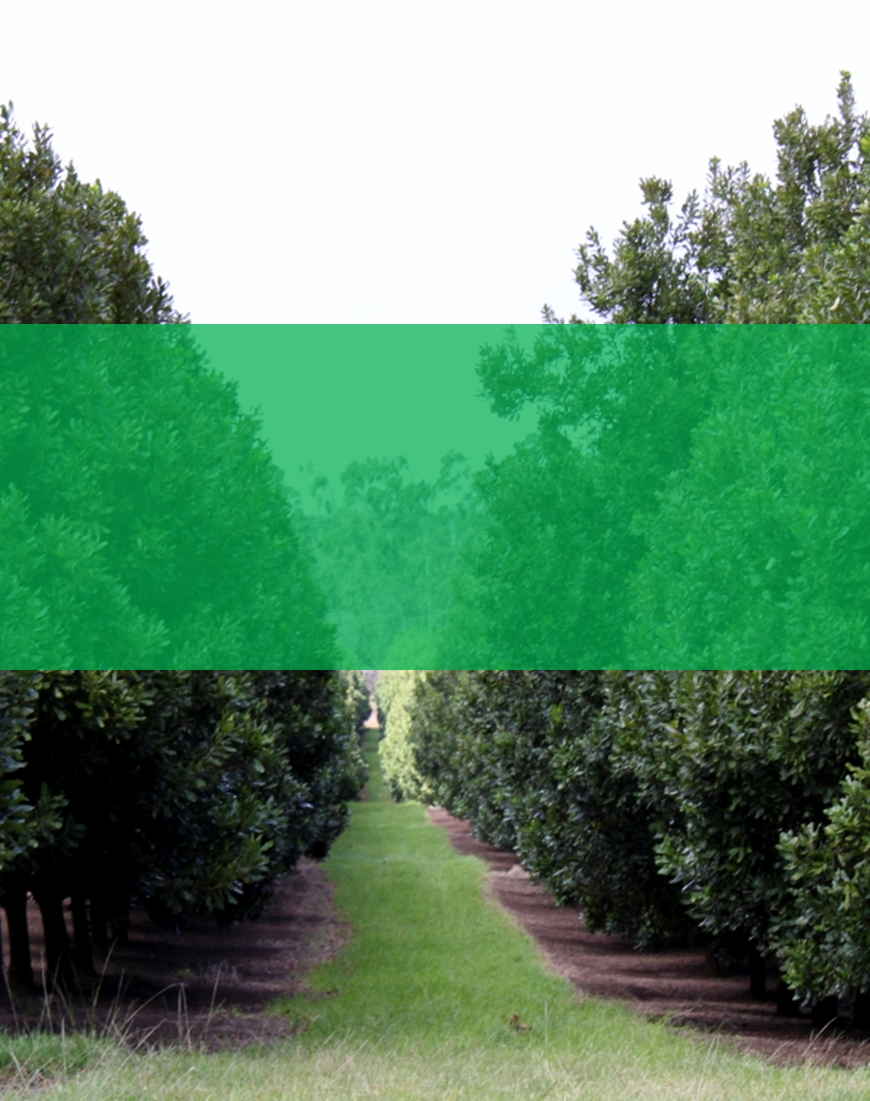
\includegraphics[scale=1]{frontcover}}} % Image background
	\centering
	\vspace*{5cm}
	\par\normalfont\fontsize{35}{35}\sffamily\selectfont
	\textbf{Harvest}\\
	{\LARGE Software Architectural Requirements and Design}\par % Book title
	\vspace*{0.5cm}
	{\Huge HTTP\_418}\par
	\centering
	\vspace*{0.5cm}
	\begin{itemize}[label={}, noitemsep]	
		\Large
		\item \begin{center} Christiaan Saaiman, 12059138 \end{center}
		\item \begin{center} Michael Loosen, 14017254 \end{center}
		\item \begin{center} Elizabeth Bode, 14310156 \end{center}
		\item \begin{center} LC Meyers, 14024633 \end{center}	
	\end{itemize}
	\endgroup
	
	%----------------------------------------------------------------------------------------
	%	TABLE OF CONTENTS
	%----------------------------------------------------------------------------------------
	
	\chapterimage{orchard.png} % Table of contents heading image
	
	\pagestyle{empty} % No headers
	
	\tableofcontents % Print the table of contents itself
	
	%\cleardoublepage % Forces the first chapter to start on an odd page so it's on the right
	
	\pagestyle{fancy} % Print headers again
	
	%----------------------------------------------------------------------------------------
	%	CHAPTER 1
	%----------------------------------------------------------------------------------------
	
	\chapterimage{mangoes.png} % Chapter heading image
	
	\chapter{Vision}
		The client, Subtrop, has requested that we implement a system to keep track of the crop yields of farms registered with them. The scope of the system entails managing the administration involved in the tracking of yields and the performance of the farm workers. Currently, this is done by manual tracking on a paper-based system. The system is required to keep track of all yield data and the associated farm’s metadata.\newline\newline
		The current paper-based system consists of various farmers, their farms, the foreman they have appointed, their workers that work under the foreman and the different Subtrop crop type associations. Farms are divided into orchard blocks with each block having one crop type associated with it. Workers are paid according to their performance and, thus, this data has to be recorded. These two factors provide the potential for statistical data reports, which could aid farmers in strategic decision-making.\newline\newline
		The most fundamental requirements that the client would like the system to fulfil are:
	\begin{itemize}
		\item Keeping track of yield data in order to see which orchards are successful
		\item Keeping track of worker performance in order to ensure that they are working to their full potential
	\end{itemize}

	
	
	%----------------------------------------------------------------------------------------
	%	CHAPTER 2
	%----------------------------------------------------------------------------------------
	\chapterimage{macadamias.png}
	
	\chapter{Background}
	\begin{itemize}
		\item Limitations of current system\newline\newline
		The current system being used by the client involves manually tracking worker performance with the use of a clipboard, with a list of all the workers names, and a pen.  The farmers have to manually record every yield that each worker collects in order to track their performance to determine their wages. The current system is inefficient due to the tedious nature of it. This tediousness reduces the foreman’s productivity as time is wasted unnecessarily searching for workers in the list and keeping track of all the lists chronologically. As the foreman is in charge of the workers, the workers have to wait until the yield they collected has been recorded which in turn also reduces their productivity.\newline
		
		\item High theft issue\newline\newline
		Farmers in the subtropical growers industry are continuously burdened by theft of their products by their own employees. This results in decreased revenue, increased costs, reduced productivity and a decrease in employer-employee trust, which creates the potential for a poor working environment. All of which necessitates the development of a new system that seeks to reduce the probability of crime by implementing monitoring on the foreman’s devices.\newline
		
		\item Need for statistical data\newline\newline
		The potential for generating statistical data that could aid farmers in future decisions from the manual data they collect is immense. The current paper-based storage of data prevents the generation of statistical reports due to the immense workload and time it requires. There is a huge need for reports indicating the highest producing orchard blocks, appropriate allocation of orchard block conditions to crop types and expected revenue. All of which could assist the farmers in future strategic planning.
	\end{itemize}
	%----------------------------------------------------------------------------------------
	%	CHAPTER 3
	%----------------------------------------------------------------------------------------
	
	\chapterimage{avocados.png}
	\chapter{Architecture Requirements}
	
	\section{Architectural Scope}
		We at HTTP\_418 have taken a philosophy of quality work. Therefore we have decided to create an application that is centralised around a few core ideas. This ideology will drive us to create an application for Subtrop as best as we can.\newline
		We will work in a persistence framework because we recognise our client’s need to have accurate, reliable data on hand when necessary. Our framework relies on databases, with integration for any database, meaning that if we wish to switch from a SQL to a NoSQL database, we will be able to do so. Alongside this, our design will incorporate security with regards to accessing the data stored. We will also be making use of techniques and technologies that will allow us to persistently add and remove data with concurrent accesses to the database.\newline
		Our system will also feature a reporting aspect that will be characterised as central, independant, consistent \& accurate as well as timely \& reliable. The independence is a key feature such that a report can still be generated in the event that the rest of the system is experiencing problems.\newline
		Our system will be accessible on the client-side via a desktop web client as well as an application on Android Mobile. The web client will have greater functionality than the Android application as it will serve as an admin/control interface where the user is able to manage the system, update details and view statistics. The Android Application will merely provide basic functionality for data input and throughput.\newline
		The system will also require real-time updates. As the gatherers hand in their pickings and the foreman enters them on the application, the farmer must be able to view/track the changes from his web client.\newline
		Our system is also be required to produce heat maps. These are graphical representations of the yield that a certain area delivers. They are created using the data stored in our database.\newline
		Our system will be used in excess of 900 farmers and a much greater number of foreman, meaning that there will be a great emphasis on scalability, performance and reliability. \newline
		Lastly we would like to create the system in such a way that a user is able to add and remove modules without it necessary to shut the system down.\newline
	\section{Access Channel Requirements}
		The access channels can be divided into two sections, namely Human and System.\newline
	\subsection{Human Access Channels}
		The user will be able to access the system through two channels, namely a web client interface and an Android application interface.\newline
		The web client interface will be strictly reserved for the farmers with which they can interact with the system in a superuser sense. The farmer will be able to assign workers to each foreman and in real time track the progress of his harvest, each worker’s statistics, the foreman’s location as well as view statistics on his harvests and view a heat map.\newline
		The Android application will have limited functionality. It will be used by the foreman’s while they are out with the harvesters to keep track of the amount of bags that each worker brings in. It will be made available on the Google PlayStore and will run any device running Android 4.0 or higher.\newline

	\subsection{System Access Channels}
		Our framework that we chose, namely SailsJS makes RESTful architecture easy and simple. Sails uses the RESTful API to already REST wrap all our objects. Along with that, SailsJS features Waterline, an intuitive interface for any 	database we would like to use, from MongoDB to PostgreSQL.\newline
	
	\section{Quality Requirements}
		There are many quality requirements for an application such as ours. Here we will look at them and in short discuss them.\newline
		\subsection{Performance}
			\subsubsection{Description}
				Application performance is measured as amount of work done within a certain time period. Our job as developers is to get as much done as quickly possible without sacrificing integrity, security and Reliability.\newline
			\subsubsection{Justification}
				The more work can be accomplished by the usage of this application, the more productive farmers can be in other areas and the better they can use the data to determine where to apply fertiliser etc.\newline
			\subsubsection{Requirements}
				\begin{itemize}
					\item Network requests must be benchmarked, monitored and aggregate statistics about network requests must be made available.
					\item Function calls must be timed and benchmarked and this data should be logged.
					\item Network responses should be cached on server side to lighten the load on database as well as decreasing the round trip time of request - response.
				\end{itemize}
		\subsection{Reliability}
			\subsubsection{Description}
				The system we are developing must be reliable in its data persistence and accessibility. System crashes and data loss is not acceptable in any circumstance.
			\subsubsection{Justification}
				The preservation of data is extremely important for every farmer seeing as this data will be converted into valuable information used to create reports and heat maps.
			\subsubsection{Requirements}
			\begin{itemize}
				\item To enable offline activity and access of data from the Android app, data synced must be made differentiable with timestamps.
				\item The system must resolve synchronization conflicts using timestamps.
				\item Hot swapping of system modules should not affect system service reliability.
			\end{itemize}
		\subsection{Scalability}
			\subsubsection{Description}
				Scalability is the application’s ability to handle above normal workloads. Our client has specified the estimate of number of users for our application, however we will cater for for a larger number not to only be safe, but to also cover the possibility of rapid expansion.
			\subsubsection{Justification}
				Our application requires scalability due to the large number of farmers that will be using this application. An estimate of in excess of 900 farmers, each with multiple foreman will make use of it.
			\subsubsection{Requirements}
				\begin{itemize}
					\item The application must be able to cater for more than 900 farmers each with multiple foreman each.
					\item The application must be able to handle multiple concurrent sessions
				\end{itemize}
		\subsection{Security}
			\subsubsection{Description}
				Security in terms of software applications is referred to authentication, authorization, data security \& accounting. Authentication is the ability of our application to identify a user using the application. Authorization is the level of authority that an authenticated user has to execute commands. Data security has to do with our application’s data only being accessible through secure channels and accounting refers to the fact that a user’s actions and effects on the system can be traced and accounted to them.
			\subsubsection{Justification}
				Security is one of the most important features in today’s age, the Information Age. Information is power. We are concerned about the user’s data integrity, availability, confidentiality and accountability.\newline
				Our reason for our worry about data integrity is because the user will be using the data he gathers to determine how to proceed further with his/her business. Real time data analysis and viewing will be a key aspect of our application, so we need to make sure that the integrity of that data is to be trusted.\newline
				We want to be sure that the user that uses this application does not have access to other user’s details and statistics and along with this we want accountability for the users who do use this application and bring changes to the database.
			\subsubsection{Requirements}
				\begin{itemize}
					\item User access rights will be checked against the database and depending on the level of clearance, a different user interface will be populated.
					\item The Android application’s user authentication details should not be stored on the Android device itself, but on the server so that the service of the application can be denied if the need arises.
					\item Passwords and unique salts should be used for each user.
					\item If a user attempts to access his user account and fails to enter the correct password x amount of times, the account should be locked and require a superuser to unlock it.
					\item Access to the database should require authentication
				\end{itemize}
		\subsection{Flexibility}
			\subsubsection{Description}
				Flexibility is the application’s ability to be changed dynamically either via a plugin for extension or otherwise.
			\subsubsection{Justification}
				Flexibility is necessary for any application to be successful, otherwise it would mean that the application was hardcoded to only work in a certain manner on a certain machine. It is also necessary that when changes need to be made, that as little as the as possible is influenced in the system and needs to be changed. A flexible system is also easier maintain and repair.
			\subsubsection{Requirements}
				\begin{itemize}
					\item The system should allow unregistered users to use existing third party web service login credentials to register or login to the service.
					\item The system should be decoupled from the database technology it uses and allow the client to select and change the database it uses in future.
					\item Authentication mechanisms used should be decoupled from the system, allowing them to be interchangeable.
					\item Modules should be decoupled from one another, allowing the system to be extensible without a break in service which is achieved by integrating new modules and swapping out existing ones.
				\end{itemize}
		\subsection{Maintainability}
			\subsubsection{Description}
				The system is to be designed in such a way that it is easily updated, modified or extended by the client in the future. In order to achieve these requirements, design patterns and best practices such as coding style guides are normally used to ensure uniformity and modularity across the system.
			\subsubsection{Justification}
				Many systems require regular changes, not because they were poorly designed or implemented, but because of changes in external factors.
			\subsubsection{Requirements}
				\begin{itemize}
					\item Code should be documented in the applicable language documentation framework.
					\item A coding style should be agreed upon between all the developers so that the same style is used throughout and the same terminology is applied.
					\item The application should be clearly separated into clear and concise modules to divide concerns and allow for easier maintenance.
				\end{itemize}
		\subsection{Auditability/Monitorability}
			\subsubsection{Description}
				The system is to be designed to be verbose and transparent in its workings, and to ensure maximum data security, to allow role players to have insights into how the system is used and how it may be improved.\newline
				These requirements are achieved by making the maximum amount of relevant data available to authorized users, logging performance critical information, and by enforcing strict constraints on the data that is stored.
			\subsubsection{Justification}
				This is an important process in Software Engineering, where all the informations must be correct so requiring all the developers to see who made changes and when so that consistency must be kept in order to keep the database accurate and reliable.
			\subsubsection{Requirements}
				\begin{itemize}
					\item Database data should be consistent and never deleted.
					\item User creation and edit times should be visible.
					\item Keep an immutable log of user actions.
					\item Logging of stack traces and crash analytics should be implemented.
				\end{itemize}
		\subsection{Integrability}
			\subsubsection{Description}
				The system should allow for future external integration with other platforms such as security authentication providers, other external research metadata databases etc.
			\subsubsection{Justification}
				The system necessitates integrability to allow for maximum usability, as the integrability of the system is directly related to how usable it is. To be usable, the system must allow for easy migration, not just from previous systems, but also to future systems and future data storage mediums.
			\subsubsection{Requirements}
				\begin{itemize}
					\item The system should allow technology neutral importing and exporting of data.
					\item The back-end system should integrate with a desktop web client and Android mobile app clients.
					\item The system should be able to integrate with different back-end authentication services.
				\end{itemize}
		\subsection{Cost}
			\subsubsection{Description}
				The cost of the system entails any initial expenses as well as any ongoing expenses which the client may incur at some point. Such expenses arise from software licenses, external computing resources required as well as future maintenance of the system in terms of time.
			\subsubsection{Justification}
				The expenses made and software licenses cost must be taken into account in order to set the price of the software.
			\subsubsection{Requirements}
				\begin{itemize}
					\item System should be cheap to operate, maintain and extend. If the quality and maturity of technologies available allow it, technologies used must be freely available/usable.
					\item As far as possible, open source compatible, mature technologies should be used, to ensure system stability as far as possible.
				\end{itemize}
		\subsection{Usability}
			\subsubsection{Description}
				Usability refers to ease with which humans, and to a lesser extent, servers, interact with the system in question. Usability can be measured in various ways such as using quantifiable scientific measures or more subjective measures with a key question point being if the API follows conventions and so on.
			\subsubsection{Justification}
				It is important that the new system is usable as it is a user-centric system. Ensuring that the system is usable will ensure that users capture accurate and correct information into the system which will for better performance and farmer strategic planning.
			\subsubsection{Requirements}
				\begin{itemize}
					\item Each view in the desktop and mobile clients should be related to a single topic only.
					\item The web client should render properly and be fully functional in modern web browsers.
					\item Mobile devices running Android 4.0 and upwards should be fully supported.
					\item Material design UI guidelines prescribed by Google must be used, to ensure that the clients feel modern and familiar.
					\item Android app and web client should support the full back-end API specifications.
					\item The user must be allowed to elect whether they would like their data to be available offline.
					\item Mobile client users should be able choose between downloading data over Wi-Fi or 3G.
				\end{itemize}
		
	\section{Integration Requirements}
		Our web client will be usable on most modern day PCs with support for the big browsers. With the usage of SailsJS we are able to automatically incorporate RESTful APIs with our web client as well as seamless database integration.\newline
		Our Android application will focus on acquiring data and sending it once a internet connection is achieved seeing as the foreman won’t always have signal out in the orchids. We will persist the data entered locally on the phone only to upload the data later. Due to internet costs we will make sure we keep the data as small as possible and the bandwidth usage low as well. Phonegap and Ionic help with these regards.\newline

		SailsJS provides us with the necessary framework to easily achieve this. It takes care of the REST wrapping automatically and integrates with our database. It uses NodeJS and is built on top of Express, thus we are using fully JavaScript libraries everywhere.\newline
	\section{Architecture Constraints}
		The only constraints placed on us with regards to the architecture is that the client wants a web client that has a superuser functionality and an Android application. We were given free reign in our judgement on how we wish to accomplish this task. In our technologies section we discuss what we will be using and how it relates to our project.\newline
	
	%----------------------------------------------------------------------------------------
	%	CHAPTER 4
	%----------------------------------------------------------------------------------------
	
	\chapterimage{litchis.png} % Chapter heading image
	
	\chapter{Architectural Tactics or Strategies}
	
	\section{Software Engineering Context : Architectural Tactics}
		Architectural tactics is concerned with achieving coherence between a design decision and a quality response/promise. Simply put, this refers to how we plan to keep our promise of the level of quality stated previously.\newline
	\section{Performance Tactics}
	\subsection{Three Groups of Performance Tactics}
		\begin{itemize}
			\item Resource demand tactics\newline
			Simply explained, these are tactics that regulate the allocation of resources
			\item Conflict resolution tactics\newline
			These are tactics designed specifically to resolve conflicts between modules etc
			\item Multiple Resource Managements Tactics\newline
			These tactics are resposible for the mangements of concurrent resource accesses and similar tasks
		\end{itemize}
	\section{Reliability Tactics}
		Reliability of the system refers to amongst other things, the coherence of information stored within the system and presented to users(concurrent). This can be achieved through the use of a duplication scheme which can be sought after using Passive Redundancy, which simply means that the system is designed to store the same information multiple times in multiple independent locations. System reliability also refers to the systems automatic fault detection.
	\subsection{System Context}
		\begin{itemize}
			\item Offline data storage\newline
				The user is able to use the Android application even without signal and/or internet connection. The data entered into the application gets persisted locally and is later then sent to the server once the phone regains connection.
		\end{itemize}
	\section{Scalability Tactics}
	Scalability refers to the ability to handle increased workload without adding more resources to the system. One way to achieve scalability is to perform a regular SWOT analysis on the system:\newline
	–Strengths : the kinds of growth the system is designed to handle\newline
	–Weaknesses : the kinds of growth the system will have trouble handling\newline
	–Opportunities : possible changes in the system which could be exploited to increase performance\newline
	-Threats : possible changes in the workload that the system will not be able to handle
	\section{Security Tactics}
	Security refers to the protection of information systems from unauthorized disruption that could potentially result in the corruption of information. It is achieved by enforcing access controls on individuals, according to a user hierarchy, to ensure only permitted users have access to the necessary information.
	\subsection{System Context}
	\begin{itemize}
		\item Resistance to SQL injections\newline\newline
		SQL injections are dependent on data type awareness in order to be successful. To prevent this, the data being transferred will be encrypted to hide its data type so only the system can understand it. All authentication data will be stored in an encrypted form and never in plain-text.\newline
		
		\item Enforce access rights according to user hierarchy \newline\newline
		The different users of the system, such as the farmer and the foremen, will have different access rights accordingly. The farmer will be a super user and will, thus, have access to all functionality that the system offers. The foremen will be general users and have restricted access to administration functionalities. This will simply be enforced by enabling and disabling certain functionalities according to user logins.\newline
		
		\item Password encryption\newline\newline
		Upon registration of a user account, the user’s password will be stored in the database after it has been automatically hashed. When the user logs in, the hashed password will be retrieved and converted to plain-text to perform authentication. No passwords will be stored in the database in plain-text format.\newline
		
		\item Enforce database authentication\newline\newline
		Access to database queries will be limited according to the aforementioned user hierarchy. The farmer will have direct access to view and modify the database whereas the foremen will only be able to make additions to the database regarding worker performance.			
	\end{itemize}
	\section{Flexibility Tactics}
	Flexibility refers to the ability to respond to changes whether internally or externally and how the software reacts to the changes. It also describes how much changes need to be made in order to adapt to the changes.
	\subsection{System Context}
	\begin{itemize}
		\item When the mobile app is adapted to run on other platforms the system must not be changed to much and easily plug into the new platform.
		\item When a different database is chosen the system must not notice that the database is changed.
		\item When farmers from different industries start to use the service, they only need to update the system to be aware of their specific specifications for yields and other data, with minimal effort.
		\item Changes to the internal structure of the system should be adapted for with minimal effort.
	\end{itemize}
	\section{Maintainability Tactics}
	Maintainability refers to modifying the existing system to make improvements or fix bugs without jeopardizing the data integrity and functionality. The need for maintainability is usually based on the following factors: changes in the software environment, new user requirements, bug and error fixes and the requirement of preventative measures for future problems.
	\subsection{System Context}
	\begin{itemize}
		\item Enforce code documentation\newline\newline
		JSDoc will be enforced as the documentation framework as its sole purpose is to generate documentation for JavaScript, the language which the whole system will be based on. This will ensure that other developers will always be able to understand what is going on in the code.\newline
		
		\item Setup coding standards and conventions\newline\newline
		The CSS3 files should be sorted alphabetically to aid in navigation and understanding for other developers. Other good practices such as naming conventions for variables, functions and classes should be specified to ensure consistency and readability throughout.\newline
		
		\item Enforce modularization of system components\newline\newline
		The system should separate concerns by dividing the system components into distinct and independent modules to improve maintainability. This will be enforced with the use of various frameworks such as Node.js, Express,js, Sails,js and Angular.js, which require separation of concerns as they are MVC-oriented.
		
	\end{itemize}
	
	\section{Auditability Tactics}
	Refers to information about the performance of the system , and to provide a log of which user provided which input at which point in time.
	\subsection{System Context}
	\begin{itemize}
		\item Any errors thrown by the system or fatal errors made by users should be logged for security and reliability analyses.
		\item Any attacks aimed at the system should be logged if possible
		\item Data in the database should be consistent and that will be achieved by constraints put in place and validation of user input.
		\item Data in the database should never be deleted, if the user deletes data, the data will be moved to another database so that data can be recovered.
		\item Regular data backups need to be made.
	\end{itemize}
	\section{Integrability and Extensibility Tactics}
	Integrability refers to testing whether separately developed components work together correctly. Extensibility evaluation is focused on how the addition of new features can take place without losing existing features.
	\subsection{System Context}
	\begin{itemize}
		\item JavaScript will be used on the server-side and the client-side of the architecture in order to seamlessly integrate the flow of data.
		\item The back-end of the system should integrate with a Web client and the mobile applications’ clients respectively.
		\begin{itemize}
			\item This will be achieved using Sails.js as this integrates well with Node.js and can, therefore, integrate with AngularJS, which is what both the Web interface and mobile interfaces will be built in.
		\end{itemize}
		
	\end{itemize}
	
	\section{Cost Tactics}
	Costs refer to all the funding required in order for the system to function fully. These costs include development costs, operational costs and maintenance costs.
	\subsection{System Context}
	\begin{itemize}
		\item Ensure costs are kept to a minimal \newline\newline
		The chosen technologies are open-source to ensure the costs associated to the operation, maintainability and extension of the system are kept to a minimum. However, if the need arises that the system requires the incorporation of a functionality that open-source software can’t offer, then the software will be chosen according to the best value for money. Thus, development costs will be kept to a minimum. The only concerns regarding operational costs are regarding the deployment of the application onto a public exchange interface and the server. The client requires the application to be present in the Google PlayStore and the Apple AppStore, which will infer yearly costs. If the client currently has a functional server that could handle the workload of the application then the server costs won’t be an issue. Otherwise, a server will need to be bought and setup, which will result in various costs. The potential need to invest in an additional server might also occur, but this is dependent on the popularity and scalability of the system. For system development, any free open source IDE or text editor and browser can be utilized by the developers to reduce maintenance costs.
		
	\end{itemize}
	
	\subsection{Usability Tactics}
	Usability refers to the usefulness of the components that have been developed.
	\subsection{System Context}
	\begin{itemize}		
		\item The web client should be fully functional in popular Web browsers.
		\begin{itemize}
			\item The Web client must function correctly in all of the popular Web browsers in order to increase the usability, as not everyone uses the same browser.
			\item The Web client should function in older versions of the popular browsers as well, as the user may not have the latest updates installed.
		\end{itemize}
		\item Mobile devices running Android 4.0 and upwards and iOS 7 and upwards should be fully supported.
		\item The Android app and Web client should support the full back-end API specifications.
	\end{itemize}
	
	
	%----------------------------------------------------------------------------------------
	%	CHAPTER 5
	%----------------------------------------------------------------------------------------
	
	\chapterimage{farmer.png} % Chapter heading image
	
	\chapter{Reference Architectures and Frameworks}
	
	\section{Backend System}
	\subsection{Programming Languages}
	\begin{itemize}
		\item Javascript:
		\begin{itemize}
			\item \textbf{Description}\\
			Javascript is a dynamic scripting language that supports procedural or object orientated programming through use of prototypes. Javascript is the main language on which Node.js packages are written in.
			\item \textbf{Performance}\\
			Because of the fact that Javascript is a lightweight scripting language it is fairly fast and mainly depends on the performance of the javascript interpreter or runtime environment.
			\item \textbf{Flexibility}\\
			Javascript is a scripting language which means that javascript can run on anything that can interpret the javascript scripts.
			\item \textbf{Usability}\\
			Javascript can be used at the client side along with web development or it can be used on node.js to create a web server.
		\end{itemize}
	\end{itemize}
	\subsection{Frameworks}
	\begin{itemize}
		\item Node.js
		\begin{itemize}
			\item \textbf{Description}\\
			Node.js is in fact not a framework but rather a runtime environment for Javascript that enables you to create web servers by only using Javascript. Node.js is built on Google’s V8 Javascript Engine which is a very high performance Javascript interpreter built into Google Chrome and written in C++.
			\item \textbf{Performance}\\
			Node.js uses an event driven non I/O blocking model that means that no blocking will occur on the server and waiting for real time updates from a lot of connected clients will not tax the server and reduce it’s performance. This means a lot for the real time nature of our project.
			\item \textbf{Scalability}\\
			Because Node.js responds to events instead of waiting on requests like other platforms such as JavaEE typically does the server can easily be scaled to handle a huge amount of client requests. The fact that Node.js runs on an asynchronous model means that many concurrent requests will not result in long waiting times for a response.
			\item \textbf{Security}\\
			Node.js has been built with security in mind and is still actively being improved on the security front.
			\item \textbf{Flexibility}\\
			Node.js relies on packages to be added, this means that virtually anything can be achieved by including a package from the huge variety of packages available from \textbf{Node Package Manager}.	
		\end{itemize}
		\item Express.js
		\begin{itemize}
			\item \textbf{Description}\\
			Express.js is a minimal web application framework for Node.js. It supports single page, multi page and hybrid page web and mobile applications and is the de facto framework to use for Node.js based web servers.
			\item \textbf{Performance}\\
			Express.js is very minimal and therefore does not affect the performance of Node.js much.
		\end{itemize}
		\item Sails.js
		\begin{itemize}
			\item \textbf{Description}\\
			Sails.js is a MVC style framework that runs on top of Express.js. It is built to enable rapid development of server side web applications and works very well for applications that needs real time functionality.
			\item \textbf{Flexibility}\\
			Sails.js does not depend on any type of front end. It also supports any database and can support many different databases in the same project. Any database that is not supported can still be used through adapters.
			\item \textbf{Maintainability}\\
			Sails.js is designed to be coded once and just work. Therefore it is coded once and forgotten very little maintenance is needed.
			\item \textbf{Usability}\\
			Sails.js is built from the start to be very easy to use and set up. It can also create RESTful api’s for you project
		\end{itemize}
	\end{itemize}
	\subsection{Database System}
	\begin{itemize}
		\item MongoDB
		\begin{itemize}
			\item \textbf{Description}\\
			MongoDB is a popular NoSQL document-oriented database that is open-source and cross-platform. It stores data in JSON-like documents which are stored in binary form called BSON.
			\item \textbf{Performance}\\
			The structure of MongoDB provides high throughput and low latency meaning regardless of the amount of queries being executed simultaneously it performs timely and consistently.
			\item \textbf{Scalability}\\
			MongoDB can handle an increasing amount of users and queries due to its ability to scale up and scale-out by utilising automatic sharding without increased time frames. In contrast to relational databases, whereby the time takes longer as the database enlarges.
			\item \textbf{Usability}\\
			The setting up of MongoDB is generally the only challenge. However, the querying syntax is simple and easy to learn.
		\end{itemize}
	\end{itemize}
	\subsection{Operating System}
	\begin{itemize}
		\item Linux
	\end{itemize}
	\subsection{Dependency Management and Build Tools}
	\begin{itemize}
		\item NPM
		\begin{itemize}
			\item \textbf{Description}\\
			Node package manager is not only used to install new packages into the local Node repository, but it also has the added feature of managing dependencies on packages within your project.
		\end{itemize}
	\end{itemize}
	\section{Web Interface}
	\subsection{Programming Languages}
	\begin{itemize}
		\item Javascript
		\item HTML5
		\begin{itemize}
			\item \textbf{Description}\\
			HTML5 is the 5th iteration of Hyper Text Transfer Protocol. HTML is a markup language used mainly in websites to markup text into something more interesting that plain text.
			\item \textbf{Usability}\\
			HTML5 is mainly used for web pages but can also be used to design an interface in hybrid mobile apps.
		\end{itemize}
		\item CSS3
		\begin{itemize}
			\item \textbf{Description}\\
			CSS3 is the third iteration of Cascading Style Sheet. CSS itself is also a markup language. CSS is used in conjunction with HTML to mark up web pages.
			\item \textbf{Usability}\\
			CSS is used to stylise HTML text to make it more visually appealing. It can be used to color text, define spacing define image sizing and much more.
		\end{itemize}
	\end{itemize}
	\subsection{Frameworks}
	\begin{itemize}
		\item Sails.js
		\item AngularJs
		\begin{itemize}
			\item \textbf{Description}\\
			AngularJS is a Javascript framework that extends HTML5. It extends HTML DOM and makes it more responsive.
			\item \textbf{Flexibility}\\
			AngularJS most suited for application development where single page applications are mostly used. But AngularJS also works well to make normal web pages responsive. Angular is usability test ready and is linked together by Dependency Injection.
			\item \textbf{Usability}\\
			AngularJS makes it very easy to implement MVC by asking the programmer to split the project into the components and then Angular will handle the rest.
		\end{itemize}
		\item Bootstrap
		\begin{itemize}
			\item \textbf{Description}\\
			Bootstrap is a mobile-first front-end framework for websites and webapps that mainly aids in layout design of web projects.
			\item \textbf{Flexibility}\\
			Bootstrap makes websites responsive to screen sizes and automatically switches to a more mobile friendly layout when screen sizes reach a certain size. This makes it possible to code the website once for different screen sizes.
			\item \textbf{Usability}\\
			Bootstrap can be used for normal full sized websites or for sites intended for mobile devices or even for websites meant to be viewed on both screens. Bootstrap also works brilliantly for managing the layout in hybrid apps.
		\end{itemize}
	\end{itemize}
	\subsection{Libraries}
	\begin{itemize}
		\item Google Maps API
		\begin{itemize}
			\item \textbf{Description}\\
			There was no other place to put this but under frameworks, even though it is not a framework but rather an Application Programming Interface. Google Maps API is a service from Google that enables developers to embed google maps into their websites and perform operations on the embedded map.
		\end{itemize}
	\end{itemize}
	\subsection{Database System}
	\begin{itemize}
		\item MongoDB
		\item Cookies
		\begin{itemize}
			\item \textbf{Description}\\
			Cookies are a temporary method of local storage mainly used to remember user logins or user preferences on websites.
		\end{itemize}
		\item HTML5 Local Storage
		\begin{itemize}
			\item \textbf{Description}\\
			HTML5 Local Storage is a way for websites to store data on the client in a sandbox so that the stored data is only accessible by the browser that controls the sandbox.
			\item \textbf{Security}\\
			The sandbox makes sure no malicious data will make it through to any important places on the computer
			\item \textbf{Usability}\\
			There exists some local databases that take advantage of HTML5 Local Storage to make a type of offline database that can be used to store data that needs to be synced with a web database at a later stage.
		\end{itemize}
	\end{itemize}
	\subsection{Operating System}
	\begin{itemize}
		\item Device Operating System Independent
		\item Web Browser
		\begin{itemize}
			\item Google Chrome
			\item Mozilla Firefox
			\item Microsoft Internet Explorer 8,9 \& 10
			\item Microsoft Edge
			\item Apple Safari
		\end{itemize}
	\end{itemize}
	\subsection{Dependency Management and Build Tools}
	\begin{itemize}
		\item Unit.js
		\item Dagger
	\end{itemize}
	\section{Android Client}
	\subsection{Programming Languages}
	\begin{itemize}
		\item Javascript
		\item HTML5
		\item CSS
	\end{itemize}
	\subsection{Frameworks}
	\begin{itemize}
		\item Sails.js
		\item AngularJS
		\item Bootstrap
		\item Phonegap
		\begin{itemize}
			\item \textbf{Description}\\
			Phonegap is a framework that lets developers take any ordinary web development skills and make mobile apps with that knowledge.
			\item \textbf{Usability}\\
			Developers code the app in any website and the framework will convert the website into an app, it does this by running the website in some sort of implicit “web browser”.
			\item \textbf{Flexibility}\\
			The framework has support for plugins that makes more native operations possible for the hybrid app, such as being able to use the camera to take photos or use that accelerometer to take certain measurements.
		\end{itemize}
		\item Ionic
		\begin{itemize}
			\item \textbf{Description}\\
			Ionic is a hybrid mobile app development framework that includes HTML, CSS and Javascript to create native looking hybrid mobile apps.
			\item \textbf{Flexibility}\\
			Ionic is built on top of AngularJS and Phonegap to create powerful yet native hybrid apps. It is native focused which means that Ionic follows the native platform designs to build apps that look like it’s been natively developed for the platform on which the hybrid app runs.
			\item \textbf{Performance}\\
			Ionic is optimized to be fast so that your hybrid app is fast and not slow as a website.
			\item \textbf{Usability}\\
			According to the Ionic website it is easy to learn if you already know web development. On top of that you also learn AngularJS as you learn Ionic.
		\end{itemize}
	\end{itemize}
	\subsection{Libraries}
	\begin{itemize}
		\item Google Maps API
	\end{itemize}			
	\subsection{Database System}
	\begin{itemize}
		\item HTML5 Local Storage
		\item MongoDB
	\end{itemize}
	\subsection{Operating System}
	\begin{itemize}
		\item Android 4.0 (Ice cream sandwich) and up.
		\item iOS 7 and up
	\end{itemize}
	\subsection{Dependency Management and Build Tools}
	\begin{itemize}
		\item Unit.js
		\item Dagger
	\end{itemize}
	
	
	%----------------------------------------------------------------------------------------
	%	CHAPTER 6
	%----------------------------------------------------------------------------------------
	
	\chapterimage{mangoes2.png} % Chapter heading image
	
	\chapter{Access and Integration Channels}
	
	\section{Access Channels}
	
	The farmers will be able to access the system through both a Web interface, specifically designed for the farmer, and a Mobile interface with underlying web-services. The foremen will only have access to the Mobile interface. The Web interface will be accessible by navigating to the URL of the web page within the preferred web browser of the farmer. The Mobile interface will be accessible by downloading the application from the Google Play Store or the Apple AppStore and installing it on their device. Both interfaces will make use of cookies and session ID’s in order to keep the user logged in to the system to facilitate ease of use.
	
	\section{Integration Channels}
	The entire system will be implemented using a client-server architecture due to the dynamic message-passing nature of the application. However, the frameworks that we will be using to implement the required functionality are based on the Model-View-Controller architecture. Thus, it will be the effective integration of these frameworks MVC-based functionality working collaboratively as a client-server architecture. The entire system will be coded using JavaScript as it is a dynamic, versatile language that has a lot of support. This also ensures that integration between the back-end and front-end system won’t cause any serious complications. Libraries and frameworks will also be used to adapt JavaScript to be able to run on a mobile environment.\newline\newline
	Node.js will handle the server-side communication for the system as it handles real-time data transfer quickly and efficiently regardless of scalability. Express.js will be the primary web server framework to integrate with Node.js in order to handle the message-passing. Sails.js will be a fundamental framework implemented on both the front-end and back-end of the system as it offers a multitude of functionalities and primarily integrates with Node.js. The Angular.js framework will be used collaboratively with HTML5 and JavaScript to provide the required functionality. CSS3 and the Bootstrap framework will be used to handle the styling of the front-end. AJAX will potentially be used to handle the passing of any data that cannot be handled by the other abovementioned frameworks. The Google Maps JavaScript API Heatmap Layer will be incorporated into the system in order to generate the heatmap functionality that the system requires. PhoneGap and Ionic will be used together to adapt the Web interface code to run on an Android  and iOS platform.\newline\newline
	MongoDB is the chosen database for the system as it offers the advantages of both a NoSQL database and a SQL database. It effectively handles scalability without sacrificing performance. Sails.js also provides a plugin that adapts our implementation to effectively integrate with MongoDB.
	
	
	%----------------------------------------------------------------------------------------
	%	CHAPTER 7
	%----------------------------------------------------------------------------------------
	
	\chapterimage{macadamias2.png} % Chapter heading image
	
	\chapter{Technologies}
	
	\section{Backend System}
	\subsection{Programming Languages}
	\begin{itemize}
		\item JavaScript
	\end{itemize}
	\subsection{Runtime Environment}
	\begin{itemize}
		\item Node.js
	\end{itemize}
	\subsection{Frameworks}
	\begin{itemize}
		\item Express.js
		\item Sails.js
	\end{itemize}
	\subsection{Database System}
	\begin{itemize}
		\item MongoDB
	\end{itemize}
	\subsection{Server}
	\begin{itemize}
		\item Google Compute Engine
	\end{itemize}
	\subsection{Dependency Management and Test Tools}
	\begin{itemize}
		\item Unit.js
		\item Dagger
	\end{itemize}
	\section{Web Interface}
	\subsection{Programming Languages}
	\begin{itemize}
		\item HTML5
		\item CSS3
		\item JavaScript
	\end{itemize}
	\subsection{Frameworks}
	\begin{itemize}
		\item Sails.js
		\item Angular.js
		\item Google Maps JavaScript API Heatmap Layer
		\item Bootstrap
		\item AJAX
	\end{itemize}
	\subsection{Database System}
	\begin{itemize}
		\item MongoDB
		\item HTML5 Local Storage
		\item Cookies				
	\end{itemize}
	\subsection{Servers}
	\subsubsection{Reporting Server}
	\begin{itemize}
		\item jsreport				
	\end{itemize}
	\subsubsection{Web Server}
	\begin{itemize}
		\item Nginx				
	\end{itemize}
	\subsection{Browser Compatibility}
	\begin{itemize}
		\item Google Chrome
		\item Mozilla Firefox
		\item Microsoft Internet Explorer 8, 9 and 10
		\item Microsoft Edge
		\item Apple Safari						
	\end{itemize}
	\subsection{Dependency Management and Test Tools}
	\begin{itemize}
		\item Unit.js
		\item Dagger
	\end{itemize}
	\section{Android and iOS Client}
	\subsection{Programming Languages}
	\begin{itemize}
		\item JavaScript
	\end{itemize}
	\subsection{Frameworks}
	\begin{itemize}
		\item PhoneGap
		\item Ionic
		\item Sails.js
		\item Angular.js
		\item Google Maps JavaScript API Heatmap Layer
		\item Bootstrap
		\item AJAX					
	\end{itemize}
	\subsection{Database System}
	\begin{itemize}
		\item MongoDB
	\end{itemize}
	\subsection{Operating System}
	\begin{itemize}
		\item Android Version 4 (Ice Cream Sandwich) to 6 (Marshmallow)
		\item iOS 7 to 9				
	\end{itemize}
	\subsection{Dependency Management and Test Tools}
	\begin{itemize}
		\item Unit.js
		\item Dagger
	\end{itemize}
	
	%----------------------------------------------------------------------------------------
	%	CHAPTER 8
	%----------------------------------------------------------------------------------------
	
	\chapterimage{litchiTree.png} % Chapter heading image
	
	\chapter{Open Issues}
	
	\section{Database Issues}
	\begin{itemize}
		\item We recently changed our database system from Neo4j to MongoDB so we are currently moving our system over. This was due to the fact that we were having issues with getting Neo4j to work effectively and we wanted to push development rather than waste time trying to get it to work. It also wasn't the most ideal database for our system and we decided that MongoDB suits the system's capabilities.
	\end{itemize}
	
\end{document}